\documentclass[a4paper,12pt,twoside]{memoir}

% Castellano
\usepackage[spanish,es-tabla]{babel}
\selectlanguage{spanish}
\usepackage[utf8]{inputenc}
\usepackage[T1]{fontenc}
\usepackage{lmodern} % Scalable font
\usepackage{microtype}
\usepackage{placeins}
\usepackage{natbib}
\usepackage{float}

\RequirePackage{booktabs}
\RequirePackage[table]{xcolor}
\RequirePackage{xtab}
\RequirePackage{multirow}

% Links
\PassOptionsToPackage{hyphens}{url}\usepackage[colorlinks]{hyperref}
\hypersetup{
	allcolors = {red}
}

% Ecuaciones
\usepackage{amsmath}

% Rutas de fichero / paquete
\newcommand{\ruta}[1]{{\sffamily #1}}

% Párrafos
\nonzeroparskip

% Huérfanas y viudas
\widowpenalty100000
\clubpenalty100000

% Imágenes

% Comando para insertar una imagen en un lugar concreto.
% Los parámetros son:
% 1 --> Ruta absoluta/relativa de la figura
% 2 --> Texto a pie de figura
% 3 --> Tamaño en tanto por uno relativo al ancho de página
\usepackage{graphicx}
\newcommand{\imagen}[3]{
	\begin{figure}[!h]
		\centering
		\includegraphics[width=#3\textwidth]{#1}
		\caption{#2}\label{fig:#1}
	\end{figure}
	\FloatBarrier
}

% Comando para insertar una imagen sin posición.
% Los parámetros son:
% 1 --> Ruta absoluta/relativa de la figura
% 2 --> Texto a pie de figura
% 3 --> Tamaño en tanto por uno relativo al ancho de página
\newcommand{\imagenflotante}[3]{
	\begin{figure}
		\centering
		\includegraphics[width=#3\textwidth]{#1}
		\caption{#2}\label{fig:#1}
	\end{figure}
}

% El comando \figura nos permite insertar figuras comodamente, y utilizando
% siempre el mismo formato. Los parametros son:
% 1 --> Porcentaje del ancho de página que ocupará la figura (de 0 a 1)
% 2 --> Fichero de la imagen
% 3 --> Texto a pie de imagen
% 4 --> Etiqueta (label) para referencias
% 5 --> Opciones que queramos pasarle al \includegraphics
% 6 --> Opciones de posicionamiento a pasarle a \begin{figure}
\newcommand{\figuraConPosicion}[6]{%
  \setlength{\anchoFloat}{#1\textwidth}%
  \addtolength{\anchoFloat}{-4\fboxsep}%
  \setlength{\anchoFigura}{\anchoFloat}%
  \begin{figure}[#6]
    \begin{center}%
      \Ovalbox{%
        \begin{minipage}{\anchoFloat}%
          \begin{center}%
            \includegraphics[width=\anchoFigura,#5]{#2}%
            \caption{#3}%
            \label{#4}%
          \end{center}%
        \end{minipage}
      }%
    \end{center}%
  \end{figure}%
}

%
% Comando para incluir imágenes en formato apaisado (sin marco).
\newcommand{\figuraApaisadaSinMarco}[5]{%
  \begin{figure}%
    \begin{center}%
    \includegraphics[angle=90,height=#1\textheight,#5]{#2}%
    \caption{#3}%
    \label{#4}%
    \end{center}%
  \end{figure}%
}
% Para las tablas
\newcommand{\otoprule}{\midrule [\heavyrulewidth]}
%
% Nuevo comando para tablas pequeñas (menos de una página).
\newcommand{\tablaSmall}[5]{%
 \begin{table}
  \begin{center}
   \rowcolors {2}{gray!35}{}
   \begin{tabular}{#2}
    \toprule
    #4
    \otoprule
    #5
    \bottomrule
   \end{tabular}
   \caption{#1}
   \label{tabla:#3}
  \end{center}
 \end{table}
}

%
% Nuevo comando para tablas pequeñas (menos de una página).
\newcommand{\tablaSmallSinColores}[5]{%
 \begin{table}[H]
  \begin{center}
   \begin{tabular}{#2}
    \toprule
    #4
    \otoprule
    #5
    \bottomrule
   \end{tabular}
   \caption{#1}
   \label{tabla:#3}
  \end{center}
 \end{table}
}

\newcommand{\tablaApaisadaSmall}[5]{%
\begin{landscape}
  \begin{table}
   \begin{center}
    \rowcolors {2}{gray!35}{}
    \begin{tabular}{#2}
     \toprule
     #4
     \otoprule
     #5
     \bottomrule
    \end{tabular}
    \caption{#1}
    \label{tabla:#3}
   \end{center}
  \end{table}
\end{landscape}
}

%
% Nuevo comando para tablas grandes con cabecera y filas alternas coloreadas en gris.
\newcommand{\tabla}[6]{%
  \begin{center}
    \tablefirsthead{
      \toprule
      #5
      \otoprule
    }
    \tablehead{
      \multicolumn{#3}{l}{\small\sl continúa desde la página anterior}\\
      \toprule
      #5
      \otoprule
    }
    \tabletail{
      \hline
      \multicolumn{#3}{r}{\small\sl continúa en la página siguiente}\\
    }
    \tablelasttail{
      \hline
    }
    \bottomcaption{#1}
    \rowcolors {2}{gray!35}{}
    \begin{xtabular}{#2}
      #6
      \bottomrule
    \end{xtabular}
    \label{tabla:#4}
  \end{center}
}

%
% Nuevo comando para tablas grandes con cabecera.
\newcommand{\tablaSinColores}[6]{%
  \begin{center}
    \tablefirsthead{
      \toprule
      #5
      \otoprule
    }
    \tablehead{
      \multicolumn{#3}{l}{\small\sl continúa desde la página anterior}\\
      \toprule
      #5
      \otoprule
    }
    \tabletail{
      \hline
      \multicolumn{#3}{r}{\small\sl continúa en la página siguiente}\\
    }
    \tablelasttail{
      \hline
    }
    \bottomcaption{#1}
    \begin{xtabular}{#2}
      #6
      \bottomrule
    \end{xtabular}
    \label{tabla:#4}
  \end{center}
}

%
% Nuevo comando para tablas grandes sin cabecera.
\newcommand{\tablaSinCabecera}[5]{%
  \begin{center}
    \tablefirsthead{
      \toprule
    }
    \tablehead{
      \multicolumn{#3}{l}{\small\sl continúa desde la página anterior}\\
      \hline
    }
    \tabletail{
      \hline
      \multicolumn{#3}{r}{\small\sl continúa en la página siguiente}\\
    }
    \tablelasttail{
      \hline
    }
    \bottomcaption{#1}
  \begin{xtabular}{#2}
    #5
   \bottomrule
  \end{xtabular}
  \label{tabla:#4}
  \end{center}
}



\definecolor{cgoLight}{HTML}{EEEEEE}
\definecolor{cgoExtralight}{HTML}{FFFFFF}

%
% Nuevo comando para tablas grandes sin cabecera.
\newcommand{\tablaSinCabeceraConBandas}[5]{%
  \begin{center}
    \tablefirsthead{
      \toprule
    }
    \tablehead{
      \multicolumn{#3}{l}{\small\sl continúa desde la página anterior}\\
      \hline
    }
    \tabletail{
      \hline
      \multicolumn{#3}{r}{\small\sl continúa en la página siguiente}\\
    }
    \tablelasttail{
      \hline
    }
    \bottomcaption{#1}
    \rowcolors[]{1}{cgoExtralight}{cgoLight}

  \begin{xtabular}{#2}
    #5
   \bottomrule
  \end{xtabular}
  \label{tabla:#4}
  \end{center}
}



\graphicspath{ {./img/} }

% Capítulos
\chapterstyle{bianchi}
\newcommand{\capitulo}[2]{
	\setcounter{chapter}{#1}
	\setcounter{section}{0}
	\setcounter{figure}{0}
	\setcounter{table}{0}
	\chapter*{\thechapter.\enskip #2}
	\addcontentsline{toc}{chapter}{\thechapter.\enskip #2}
	\markboth{#2}{#2}
}

% Apéndices
\renewcommand{\appendixname}{Apéndice}
\renewcommand*\cftappendixname{\appendixname}

\newcommand{\apendice}[1]{
	%\renewcommand{\thechapter}{A}
	\chapter{#1}
}

\renewcommand*\cftappendixname{\appendixname\ }

% Formato de portada
\makeatletter
\usepackage{xcolor}
\newcommand{\tutor}[1]{\def\@tutor{#1}}
\newcommand{\course}[1]{\def\@course{#1}}
\definecolor{cpardoBox}{HTML}{E6E6FF}
\def\maketitle{
  \null
  \thispagestyle{empty}
  % Cabecera ----------------
\noindent
\includegraphics[width=\textwidth]{cabecera}\vspace{1cm}%
  \vfill
  % Título proyecto y escudo informática ----------------
  \colorbox{cpardoBox}{%
    \begin{minipage}{.8\textwidth}
      \vspace{.5cm}\Large
      \begin{center}
      \textbf{TFG del Grado en Ingeniería Informática}\vspace{.6cm}\\
      \textbf{\LARGE\@title{}}
      \end{center}
      \vspace{.2cm}
    \end{minipage}

  }%
  \hfill\begin{minipage}{.20\textwidth}
    
\includegraphics[width=\textwidth]{escudoInfor}
  \end{minipage}
  \vfill
  % Datos de alumno, curso y tutores ------------------
  \begin{center}%
  {%
    \noindent\LARGE
    Presentado por \@author{Lucas Olmedo Díez}\\ 
    en Universidad de Burgos --- \@date{}\\
    Tutor: \@tutor{Carlos López Nozal}\\
    %Tutor empresarial: \@tutorempresarial{Miguel Alejandro García Bilbao}\\
  }%
  \end{center}%
  \null
  \cleardoublepage
  }
\makeatother

\newcommand{\nombre}{Lucas Olmedo Díez} %%% cambio de comando
\newcommand{\nombreTutor}{Carlos López Nozal} %%% cambio de comando

% Datos de portada
\title{Asistente de prácticas ágiles para repositorios en GitHub}
\author{Lucas Olmedo Díez}
\tutor{Carlos López Nozal}
\date{Junio de 2025}

\begin{document}

\maketitle


\newpage\null\thispagestyle{empty}\newpage


%%%%%%%%%%%%%%%%%%%%%%%%%%%%%%%%%%%%%%%%%%%%%%%%%%%%%%%%%%%%%%%%%%%%%%%%%%%%%%%%%%%%%%%%
\thispagestyle{empty}


\noindent
\includegraphics[width=\textwidth]{cabecera}\vspace{1cm}

\noindent D. \nombreTutor, profesor del departamento de ingeniería informática, área de nombre área.

\noindent Expone:

\noindent Que el alumno D. \nombre, con DNI 71306075A, ha realizado el Trabajo final de Grado en Ingeniería Informática titulado "Asistente de prácticas ágiles para repositorios en GitHub". 

\noindent Y que dicho trabajo ha sido realizado por el alumno bajo la dirección del que suscribe, en virtud de lo cual se autoriza su presentación y defensa.

\begin{center} %\large
En Burgos, {\large Junio 2025}
\end{center}

\vfill\vfill\vfill

% Author and supervisor
\begin{center}
  Vº. Bº. del Tutor:\\[2cm]
  D. Carlos López Nozal
  \end{center}
\hfill
\begin{minipage}{0.45\textwidth}
\begin{flushleft} %\large
\end{flushleft}
\end{minipage}
\hfill

\vfill

% para casos con solo un tutor comentar lo anterior
% y descomentar lo siguiente
%Vº. Bº. del Tutor:\\[2cm]
%D. nombre tutor


\newpage\null\thispagestyle{empty}\newpage




\frontmatter

% Abstract en castellano
\renewcommand*\abstractname{Resumen}
\begin{abstract}
Las prácticas ágiles han demostrado ser fundamentales en el desarrollo de software, ya que promueven la entrega iterativa, la mejora continua y una mejor colaboración entre los desarrolladores. Su aplicación es observable en los repositorios open source de plataformas como GitHub, que facilitan la gestión del código, la documentación y la colaboración entre desarrolladores. En el contexto académico, GitHub es ampliamente utilizado por los estudiantes para la gestión de sus Trabajos de Fin de Grado (TFG). Sin embargo, muchos enfrentan dificultades para aplicar correctamente las prácticas ágiles en sus repositorios, lo que puede afectar la calidad y eficiencia de su desarrollo.
El objetivo de este trabajo es ayudar a los estudiantes a aplicar prácticas ágiles en sus repositorios de GitHub mediante una aplicación web que evalúa su grado de adopción. Para ello, la aplicación analiza el uso del repositorio según consultas y reglas basadas en prácticas ágiles, comparando los resultados con valores de referencia fijos o con repositorios seleccionados como modelo.
De esta manera, la herramienta facilita la identificación de áreas de mejora y fomenta la adopción de buenas prácticas en la gestión y desarrollo de proyectos académicos en GitHub. La aplicación web está escrita en Node js y Angular y se puede acceder a su despliegue mediante la siguiente URL: 
https://gii-tfg-asistente-de-practicas-agiles-para-repositor-idxbpcutk.vercel.app.


\end{abstract}

\renewcommand*\abstractname{Descriptores}
\begin{abstract}
Métricas de calidad, proceso de desarrollo de software, prácticas ágiles, documentación continua, GitHub, análisis de repositorios.
\end{abstract}

\clearpage

% Abstract en inglés
\renewcommand*\abstractname{Abstract}
\begin{abstract}
Agile practices have proven to be essential for software development. This is because they promote iterative delivery, continuous improvement, and better collaboration between developers. Its usage is visible in open source repositories from platforms like GitHub, which make code administration, documentation, and collaboration between developers much easier. In the academic context, GitHub is heavily used by students for their TFG's administration. However, many of them face difficulties to apply correctly agile methodology in their projects, which can affect their developments' quality and efficiency. The objective of this project is to help students apply agile practices in their GitHub repositories by a web app that evaluates  the usage of agile methodology. To achieve that, the app analyzes the use of the repository using queries and rules based on agile practices, comparing results with fixed reference values or repositories selected as a comparison source. This way, the tool helps the user identify areas of improvement, and encourages the user adopting agile practices in their academic GitHub's projects' administration and development. The web app is written in Node js and Angular, and can be acceded to its deployment via the next URL:
https://gii-tfg-asistente-de-practicas-agiles-para-repositor-idxbpcutk.vercel.app.
\end{abstract}

\renewcommand*\abstractname{Keywords}
\begin{abstract}
Evolution metrics, software developing process, agile practices, continuous documentation, GitHub, repository analysis.
\end{abstract}

\clearpage

% Indices
\tableofcontents

\clearpage

\listoffigures

\clearpage

\listoftables
\clearpage

\mainmatter
\capitulo{1}{Introducción}

El desarrollo de software es un proceso complejo que involucra múltiples factores técnicos y organizativos. En el ámbito técnico, es fundamental garantizar el cumplimiento de los requisitos funcionales y no funcionales, tales como mantenibilidad, escalabilidad, eficiencia y calidad del código\cite{isoiec25000}. A nivel organizativo, la gestión efectiva de equipos de desarrollo, la planificación de tareas y la optimización del tiempo y recursos son aspectos clave para el éxito de un proyecto. Para abordar esta complejidad, se han desarrollado metodologías y herramientas que facilitan la gestión del proceso de desarrollo, promoviendo la colaboración y la mejora continua.

Las prácticas ágiles, como Scrum\cite{sutherland2014scrum}, Kanban\cite{roe2017kanban} y eXtreme Programming\cite{beck2004extreme}, han demostrado ser eficaces para gestionar proyectos de software de manera flexible e iterativa. Estas prácticas enfatizan la entrega incremental de valor, la integración continua, la colaboración entre equipos y la adaptación constante a los cambios en los requisitos del proyecto. En este contexto, la gestión de repositorios de código, como GitHub y GitLab, desempeña un papel crucial al proporcionar funcionalidades avanzadas para el control de versiones, la gestión de \textit{issues}, la revisión de código y la automatización de flujos de integración y despliegue continuo.

Sin embargo, la gran cantidad de datos generados en los repositorios de software dificulta la evaluación de la calidad del desarrollo y la documentación de este, así como la identificación de áreas de mejora. 

Diversos estudios han explorado la evaluación y aplicación de buenas prácticas ágiles en entornos de desarrollo de software. Por ejemplo, el trabajo de Chen, Chen y Hsueh (2024)\cite{Chen2024} analiza cómo la integración de prácticas ágiles en la enseñanza del desarrollo de software mejora la organización y gestión de proyectos a través del uso de plataformas como GitHub. Su estudio destaca la importancia de la gestión de \textit{issues} y \textit{commits} como indicadores clave del rendimiento de los desarrolladores, así como el papel de las herramientas automatizadas en la evaluación del trabajo en equipo y la documentación del código. Además, enfatizan que el aprendizaje basado en proyectos (\textit{Project-Based Learning}, PBL) y la incorporación de prácticas ágiles permiten mejorar la capacidad de los estudiantes para abordar problemas complejos y adaptarse a entornos cambiantes. Estos hallazgos refuerzan la necesidad de implementar sistemas que analicen y promuevan el uso de buenas prácticas en repositorios de software, alineándose con el enfoque propuesto en este proyecto para mejorar la calidad del desarrollo mediante métricas objetivas y recomendaciones basadas en prácticas ágiles.

Además, investigaciones recientes han demostrado el impacto positivo de GitHub en la enseñanza de prácticas ágiles y en el desarrollo colaborativo de software. Raibulet y Arcelli Fontana (2018) \cite{raibulet2018409} describen una experiencia en la que estudiantes de ingeniería de software participaron en proyectos colaborativos utilizando GitHub como plataforma de desarrollo. En este estudio, los estudiantes trabajaron en equipos aplicando principios ágiles y emplearon herramientas como SonarQube para evaluar la calidad del software. Los resultados evidenciaron que el uso de GitHub no solo mejoró la gestión del código y la colaboración entre los participantes, sino que también facilitó la integración de buenas prácticas de desarrollo en un entorno educativo. Estos hallazgos refuerzan la relevancia y necesidad de proporcionar herramientas que analicen y promuevan el uso de prácticas ágiles en proyectos de software, alineándose con los objetivos de este TFG.

En respuesta a esta necesidad, este TFG propone el desarrollo de una aplicación web que analiza la información de un repositorio de GitHub y, mediante la aplicación de buenas prácticas ágiles y métricas de calidad, ofrece asistencia a los desarrolladores para mejorar su proceso de trabajo.

El recurso bibliográfico S\textit{ubway Map to Agile Practices} \cite{agileSubwayMap}, desarrollado por \textit{Agile Alliance}, recopila un conjunto de prácticas ágiles ampliamente utilizadas en la industria del software para mejorar la eficiencia y la calidad en el desarrollo de proyectos. Agile Alliance es una organización global sin ánimo de lucro dedicada a promover y difundir los valores y principios ágiles, proporcionando recursos, estudios y guías que facilitan la adopción de estas prácticas en diversos entornos de trabajo. Entre las prácticas ágiles destacadas en esta colección se encuentran la integración continua, la revisión de código, las retrospectivas y la gestión visual del trabajo, todas ellas orientadas a optimizar la colaboración y el flujo de desarrollo. Basándose en estas prácticas, el sistema desarrollado en este proyecto evaluará métricas de calidad de proceso del proceso de desarrollo, como la velocidad de trabajo (frecuencia de \textit{commits} e \textit{issues} cerradas), la documentación continua, la calidad de la documentación en \textit{commits} e \textit{issues} (uso de descripciones, etiquetas y herramientas de documentación) y la implementación de pruebas automatizadas. Para ello, se emplearán métricas cuantitativas que permitirán visualizar el rendimiento del equipo y la evolución del proyecto a lo largo del tiempo, ofreciendo recomendaciones que fomenten la mejora continua y la adopción de buenas prácticas ágiles.

Este proyecto busca facilitar la adopción de prácticas ágiles y mejorar la calidad del software y su documentación mediante la automatización del análisis de repositorios. A través de este enfoque, los equipos de desarrollo podrán optimizar sus procesos, mejorar la colaboración y garantizar la entrega de software más robusto y bien documentado.

En el contexto docente de los Trabajos de Fin de Grado (TFG), las recomendaciones generadas por la aplicación pueden clasificarse en diferentes reglas de prácticas ágiles según su aplicabilidad y alcance. Se incluyen:

\textit{Automated Build}, \textit{Version Control}, \textit{Continuous integration}, \textit{Definition of Done}, \textit{Backlog Quality}, \textit{Iterations}, \textit{Velocity}, \textit{Frequent releases}, \textit{Collective Ownership} y \textit{Pair Programming}.
\capitulo{2}{Objetivos del proyecto}

Este apartado explica de forma precisa y concisa cuales son los objetivos que se persiguen con la realización del proyecto. Se puede distinguir entre los objetivos marcados por los requisitos del software a construir y los objetivos de carácter técnico que plantea a la hora de llevar a la práctica el proyecto.

\capitulo{3}{Conceptos teóricos}

En este apartado se exponen los principales conceptos teóricos necesarios para comprender el funcionamiento y objetivos del proyecto \textit{Asistente de prácticas ágiles para repositorios en GitHub}, desde los fundamentos del control de versiones y GitHub, hasta las metodologías ágiles y métricas de calidad en el desarrollo software.

\section{Control de versiones de repositorios en GitHub}
El control de versiones es una práctica fundamental en el desarrollo de software moderno, ya que permite llevar un registro completo y detallado de los cambios realizados en el código fuente a lo largo del tiempo. Entre los distintos sistemas existentes, Git se ha consolidado como el más popular gracias a su eficiencia, flexibilidad y enfoque distribuido. Este enfoque significa que cada desarrollador posee una copia completa del historial del proyecto, lo que permite trabajar de forma autónoma y sin depender de una conexión constante a un servidor central.

GitHub, por su parte, es una plataforma de desarrollo colaborativo basada en Git que añade funcionalidades adicionales orientadas a la gestión de proyectos, la colaboración remota y la revisión de código. GitHub proporciona una interfaz web amigable que facilita la visualización del historial, la discusión de cambios y la organización del trabajo en equipo. Entre sus funcionalidades clave destacan:

\begin{itemize}
\item Repositorios y ramas: Permiten organizar el código en estructuras jerárquicas y paralelas. Las ramas facilitan el desarrollo simultáneo de nuevas funcionalidades o corrección de errores sin interferir con el código principal.
\item Issues: Herramienta integrada para el seguimiento de tareas, errores y solicitudes de mejora. Facilitan la comunicación entre los miembros del equipo y permiten priorizar el trabajo pendiente.
\item Pull requests (PRs): Mecanismo para proponer y discutir cambios antes de su integración en la rama principal. Incluyen herramientas de revisión de código y validación automática mediante tests o workflows.
\item Releases: Etiquetas versionadas que marcan hitos importantes del software, como entregas estables o versiones beta. Permiten identificar fácilmente el estado de madurez del proyecto.
\item Estadísticas y métricas de calidad de proceso: GitHub ofrece paneles con datos sobre actividad reciente, contribuciones individuales, frecuencia de commits, entre otros indicadores clave del desarrollo del proyecto.
\end{itemize}

El análisis automático de estas funcionalidades y datos permite extraer información objetiva sobre la calidad, salud y evolución de un proyecto software. Esto es especialmente útil para evaluar repositorios de forma sistemática, identificar buenas prácticas o detectar áreas que requieren atención.

El análisis automático de estas métricas permite extraer conclusiones sobre la calidad, salud y evolución de un proyecto software.

\section{Métricas de calidad de repositorios}
Evaluar la calidad de un repositorio de software no solo implica revisar el código, sino también analizar cómo se gestiona y se desarrolla el proyecto en su conjunto. Esta última evaluación es la que desarrolla este proyecto empleando las metodologías ágiles. Para ello, se emplean métricas cuantitativas derivadas de la actividad registrada en el repositorio, que permiten realizar una evaluación objetiva y reproducible. Algunas de las métricas más relevantes incluyen:

\begin{itemize}
\item Número medio de commits: Indica la frecuencia con la que se realizan cambios en el código. Una actividad constante sugiere un proyecto en desarrollo activo, mientras que largos periodos sin commits pueden señalar abandono o pausas.
\item Tiempo medio de cierre de issues: Mide la eficiencia en la resolución de tareas o problemas. Tiempos de respuesta cortos suelen estar asociados a una buena organización y seguimiento, mientras que los retrasos pueden indicar falta de recursos o planificación.
\item Frecuencia de publicación de releases: Refleja el ritmo de entregas del proyecto. Una cadencia regular sugiere una metodología estructurada, como la entrega incremental propia de metodologías ágiles.
\end{itemize}

Estas métricas permiten identificar patrones de trabajo, detectar cuellos de botella y sugerir mejoras conforme a las buenas prácticas del desarrollo ágil y colaborativo. Además, se pueden utilizar para monitorizar detalladamente la evolución de un mismo proyecto a lo largo del tiempo en cada apartado del repositorio.

\section{Metodologías ágiles}
Las metodologías ágiles representan un conjunto de principios y prácticas orientadas al desarrollo de software de manera iterativa, incremental y centrada en la colaboración continua entre los miembros del equipo y con los clientes. Frente a los modelos tradicionales, como el ciclo en cascada, las metodologías ágiles fomentan la adaptabilidad, la retroalimentación constante y la entrega temprana de valor.

Dentro del universo ágil destacan marcos de trabajo como Scrum o Extreme Programming (XP), que han sido adoptados ampliamente en la industria. Estos marcos establecen roles, eventos y artefactos que ayudan a estructurar el trabajo y mejorar la comunicación del equipo. En este proyecto, se siguen principios inspirados en la guía \cite{agileSubwayMap}, la cual agrupa diversas prácticas ágiles aplicables al desarrollo de software. Entre las más relevantes se encuentran:

\begin{itemize}
\item Iteraciones y retrospectivas: Ciclos de trabajo cortos y repetitivos (sprints) al final de los cuales se evalúa lo realizado y se planifican mejoras para el siguiente ciclo.
\item Historias de usuario y definición de “Hecho”: Las historias de usuario representan funcionalidades desde el punto de vista del usuario. La definición de “Hecho” asegura que todo el equipo tiene un criterio común sobre cuándo una tarea está completada.
\item Integración continua y revisión de código: Prácticas técnicas que permiten detectar errores tempranamente, asegurar la calidad del código y facilitar la colaboración mediante herramientas automatizadas y revisiones cruzadas entre desarrolladores.
\item Visibilidad del trabajo en curso: Uso de herramientas como tableros Kanban, issues o sistemas de gestión de tareas para proporcionar una visión clara y compartida del estado del proyecto.
\end{itemize}

La aplicación desarrollada analiza la actividad del repositorio para comprobar si estas prácticas están siendo implementadas correctamente. Para ello, aplica un conjunto de reglas automáticas y sugerencias inteligentes, evaluando tanto la estructura del repositorio como su dinámica de trabajo. Esto permite no solo diagnosticar el grado de alineación con metodologías ágiles, sino también fomentar la mejora continua en la gestión de proyectos software.

\section{Análisis temporal y evaluación del proceso}
Una de las principales innovaciones que ofrece la aplicación es la incorporación de un análisis temporal personalizado, que permite estudiar cómo evoluciona el proceso de desarrollo a lo largo del tiempo. Esta funcionalidad permite seleccionar intervalos temporales específicos (como un rango de meses determinado) o relativos (por ejemplo, la primera mitad del proyecto, el tercer cuarto, etc), y aplicar las métricas correspondientes exclusivamente a ese periodo. Este tipo de análisis temporal posibilita una evaluación dinámica y contextualizada del desarrollo del proyecto.

Entre los principales beneficios de este enfoque se encuentran:

\begin{itemize}
\item Evaluación de la evolución de la calidad del repositorio: Al observar cómo cambian las métricas a lo largo del tiempo, es posible identificar tendencias positivas o negativas en aspectos como frecuencia de commits, resolución de issues o participación del equipo.
\item Análisis del impacto de cambios metodológicos: Se pueden estudiar los efectos de la introducción de nuevas prácticas de gestión, como la adopción de Scrum, integración continua o tableros Kanban, evaluando cómo influyen en la actividad y organización del equipo.
\item Medición de la madurez y estabilidad del equipo de desarrollo: Los equipos que evolucionan positivamente tienden a mostrar una estabilización en sus métricas, una mejor distribución del trabajo y un incremento en la colaboración. Estas señales permiten inferir el grado de madurez del equipo.
\end{itemize}

Este análisis es especialmente útil en contextos formativos, como el seguimiento de proyectos académicos en la Universidad de Burgos. En estos casos, permite a los tutores y alumnos evaluar el proceso de desarrollo de forma empírica, justificar la aplicación de metodologías ágiles en prácticas reales, y fomentar la reflexión crítica sobre el trabajo realizado.

\section{Evaluación de la agilidad en proyectos académicos}
El uso de la aplicación en entornos educativos proporciona una herramienta de evaluación automatizada y formativa que resulta especialmente valiosa para la enseñanza de metodologías ágiles. En particular, permite evaluar de forma objetiva y continua el grado en que los equipos de estudiantes aplican los principios ágiles en proyectos de software, como los que se desarrollan en las asignaturas de la Universidad de Burgos.

Gracias al análisis de datos extraídos directamente desde los repositorios de GitHub, la aplicación proporciona retroalimentación inmediata y personalizada a los estudiantes, permitiéndoles:

\begin{itemize}
\item Autoevaluar su desempeño: Identificando prácticas que se están aplicando correctamente y aquellas que requieren mejora.
\item Detectar deficiencias metodológicas: Como falta de actividad, ausencia de releases o escasa participación en la resolución de issues.
\item Recibir sugerencias automáticas: Basadas en reglas predefinidas y métricas objetivas, que orientan al alumno hacia una mejor implementación del enfoque ágil.
\end{itemize}

Para los docentes, esta herramienta facilita una evaluación más justa, uniforme y basada en evidencia, permitiendo valorar aspectos que habitualmente son difíciles de medir, como:

\begin{itemize}
\item Grado de implementación de marcos ágiles (como iteraciones o control de versiones), más allá de una simple declaración teórica.
\item Compromiso del equipo con las prácticas ágiles, medido a través de la participación activa y la frecuencia de interacción en el repositorio.
\item Documentación y trazabilidad del trabajo en GitHub, lo que incluye el uso de issues, descripciones de commits, pull requests revisadas, y releases etiquetadas.
\end{itemize}

Así, el análisis no solo tiene valor evaluativo, sino también educativo, ya que fomenta el aprendizaje autónomo y refuerza la comprensión de las buenas prácticas en el desarrollo ágil.

\section{Reglas de evaluación basadas en prácticas ágiles}

La aplicación analiza la actividad de un repositorio de GitHub para determinar el grado de adopción de prácticas ágiles en el desarrollo software. Para ello, se basa en 10 reglas clave inspiradas en el \textit{Subway Map to Agile Practices}~\cite{agileSubwayMap}, una recopilación de buenas prácticas organizada por familias (Scrum, Extreme Programming, DevOps, etc.).

A continuación se detallan estas reglas, su justificación y el modo en que son evaluadas por la aplicación.

\subsection{DevOps – Automated Build}

\begin{itemize}
  \item \textbf{Descripción:} El proyecto debe incluir automatización del proceso de construcción, integración o despliegue.
  \item \textbf{Criterio de evaluación:} El asistente detecta si existen ficheros de workflows (por ejemplo, bajo \texttt{.github/workflows}) que definan procesos automáticos usando GitHub Actions.
  \item \textbf{Importancia:} Favorece la repetibilidad, estandarización y reducción de errores humanos.
\end{itemize}

\subsection{DevOps – Version Control}

\begin{itemize}
  \item \textbf{Descripción:} Uso activo y adecuado del control de versiones.
  \item \textbf{Criterio de evaluación:} Se analiza la frecuencia de los commits, que estos tengan título, descripción y que estén vinculados a issues mediante \texttt{\#id} o \texttt{fixes \#id}.
  \item \textbf{Importancia:} Mejora la trazabilidad, control del código y colaboración entre miembros.
\end{itemize}

\subsection{DevOps, Extreme Programming – Continuous Integration}

\begin{itemize}
  \item \textbf{Descripción:} El repositorio debe integrar cambios frecuentemente, ejecutando pruebas automáticas.
  \item \textbf{Criterio de evaluación:} Se mide el porcentaje de éxito de los workflows automáticos, la frecuencia de su ejecución y el uso de Pull Requests para introducir cambios.
  \item \textbf{Importancia:} Detecta errores pronto y reduce conflictos al integrar código.
\end{itemize}

\subsection{Scrum – Definition of Done}

\begin{itemize}
  \item \textbf{Descripción:} Las tareas deben darse por completadas de forma inequívoca.
  \item \textbf{Criterio de evaluación:} El asistente compara el número de issues abiertas y cerradas, asegurando que las cerradas no se vuelven a abrir.
  \item \textbf{Importancia:} Establece una línea clara sobre lo que se considera terminado y entrega de valor.
\end{itemize}

\subsection{Scrum – Backlog Quality}

\begin{itemize}
  \item \textbf{Descripción:} El backlog del proyecto debe estar compuesto por issues claras, bien documentadas y priorizadas.
  \item \textbf{Criterio de evaluación:} Se comprueba que las issues tengan descripción (preferiblemente con imágenes o checklists), personas asignadas y etiquetas.
  \item \textbf{Importancia:} Permite gestionar el trabajo pendiente de forma organizada.
\end{itemize}

\subsection{Scrum, Extreme Programming – Iterations}

\begin{itemize}
  \item \textbf{Descripción:} El proyecto debe avanzar por ciclos iterativos como sprints.
  \item \textbf{Criterio de evaluación:} Se analiza si se utilizan milestones, así como la frecuencia de commits, merges y releases por ciclo.
  \item \textbf{Importancia:} Favorece la entrega frecuente de valor y mejora continua.
\end{itemize}

\subsection{Extreme Programming – Velocity}

\begin{itemize}
  \item \textbf{Descripción:} El equipo debe ser capaz de medir su velocidad de entrega de funcionalidades.
  \item \textbf{Criterio de evaluación:} Se revisa el uso de etiquetas con story points o complejidad, así como el número de issues cerradas por milestone o cada 15 días.
  \item \textbf{Importancia:} Permite planificar mejor la carga de trabajo y tomar decisiones basadas en datos.
\end{itemize}

\subsection{Extreme Programming – Frequent Releases}

\begin{itemize}
  \item \textbf{Descripción:} El proyecto debe generar versiones o releases con frecuencia.
  \item \textbf{Criterio de evaluación:} Se comprueba la existencia de releases en GitHub y la periodicidad con que se publican.
  \item \textbf{Importancia:} Permite validar funcionalidad de forma incremental y tener feedback temprano de usuarios.
\end{itemize}

\subsection{Extreme Programming – Collective Ownership}

\begin{itemize}
  \item \textbf{Descripción:} Todo miembro del equipo puede modificar cualquier parte del código.
  \item \textbf{Criterio de evaluación:} Se analiza que haya varios autores haciendo commits, revisando PRs, resolviendo issues y participando activamente en diferentes partes del repositorio.
  \item \textbf{Importancia:} Fomenta la colaboración y reduce los cuellos de botella por eExtreme Programmingertos únicos.
\end{itemize}

\subsection{Extreme Programming – Pair Programming}

\begin{itemize}
  \item \textbf{Descripción:} Los miembros colaboran en el desarrollo a través de la programación en pareja.
  \item \textbf{Criterio de evaluación:} Se detectan menciones a otros miembros en commits, PRs o issues (@usuario), así como asignaciones múltiples en tareas.
  \item \textbf{Importancia:} Mejora la calidad del código y favorece el aprendizaje mutuo.
\end{itemize}

\subsection{Resumen de reglas evaluadas por la aplicación}

\tablaSmall{Resumen de reglas ágiles evaluadas por la aplicación}{l l l}{reglasagiles}
{ \textbf{Nombre} & \textbf{Criterio evaluado} & \textbf{Práctica Agil asociada} \\ }{
Automated Build & Presencia de workflows de GitHub Actions & DevOps \\
Version Control & Frecuencia y calidad de commits & DevOps \\
Continuous Integration & Éxito y frecuencia de workflows y PRs & DevOps, XP \\
Definition of Done & Issues cerradas correctamente & Scrum \\
Backlog Quality & Calidad y estructura de issues & Scrum \\
Iterations & Uso de milestones y ciclos de commits & Scrum, XP \\
Velocity & Story points y métricas cada 15 días & XP \\
Frequent Releases & Releases frecuentes en el tiempo & XP \\
Collective Ownership & Participación múltiple en tareas y PRs & XP \\
Pair Programming & Menciones y asignaciones múltiples & XP \\
}

Estas reglas no solo ayudan a evaluar objetivamente el proceso de desarrollo de un repositorio, sino que también proporcionan a los usuarios sugerencias claras sobre cómo mejorar su adopción de prácticas ágiles.

\section{Referencias y métricas}
Las métricas y reglas empleadas por el asistente están fundamentadas en investigaciones previas y guías ampliamente reconocidas dentro del ámbito del desarrollo ágil y la ingeniería del software. En particular, se han tomado como base:

El Agile Subway Map~\cite{agileSubwayMap}, que ofrece una representación estructurada de prácticas ágiles agrupadas por niveles de madurez y propósito (por ejemplo, entrega continua, mejora del equipo, colaboración).

Estudios sobre calidad del software en entornos colaborativos, que analizan el impacto de determinadas métricas de actividad y colaboración en la sostenibilidad y efectividad de los proyectos de código abierto o académico.

Estas métricas se implementan mediante un sistema de reglas automatizadas que evalúan si ciertos umbrales se cumplen o no, y que pueden ser ajustadas según el contexto (proyecto académico, industrial, etc.). Este enfoque modular permite adaptar el análisis a diferentes necesidades, manteniendo siempre un criterio objetivo y reproducible.

\section{Resumen de herramientas utilizadas}

\tablaSmall{Herramientas y tecnologías utilizadas en cada parte del proyecto}{l c c c c}{herramientasportipodeuso}
{ \multicolumn{1}{l}{Herramientas} & Frontend & Backend & Base de Datos & Documentación \\}{
HTML5 & X & & & \\
TypeScript & X & & & \\
Angular 19.2.3 & X & & & \\
Node.js & & X & & \\
XP & & X & & \\
GitHub API & & X & & \\
Mongoose & & X & X & \\
MongoDB & & & X & \\
MongoDB Compass & & & X & \\
JWT & & X & & \\
Swagger (OpenAPI) & & X & & \\
\LaTeX{} & & & & X \\
Overleaf & & & & X \\
Git & X & X & X & X \\
}
\capitulo{4}{Técnicas y herramientas}

% Este capítulo recoge las técnicas metodológicas y herramientas utilizadas para el desarrollo del proyecto \textit{Asistente de prácticas ágiles para repositorios en GitHub}, así como las decisiones tomadas en función de las alternativas disponibles. La elección de las tecnologías ha estado guiada tanto por los requisitos funcionales del sistema como por los objetivos técnicos y personales planteados.

\section{Metodología de desarrollo}

Durante el desarrollo del proyecto se ha seguido un enfoque iterativo e incremental, inspirado en las metodologías ágiles, especialmente en la metodología \textbf{Scrum}. Aunque no se ha implementado un Scrum completo con sprints y reuniones formales, sí se ha adoptado la filosofía de desarrollo en pequeñas iteraciones, con validaciones frecuentes de funcionalidad y mejora continua.

Cada iteración se centraba en funcionalidades concretas: la recolección de datos, la visualización de medidas de proceso, el cumplimiento de las prácticas ágiles y la mejora de la experiencia de usuario. Esta división permitió avanzar progresivamente, validando en cada iteración los resultados parciales antes de pasar a la siguiente.

Además, se ha hecho uso de herramientas como \textbf{Zube} para la organización de tareas y la planificación de Issues. Esto ha facilitado el seguimiento del progreso del desarrollo.

\begin{figure}[H]
\centering
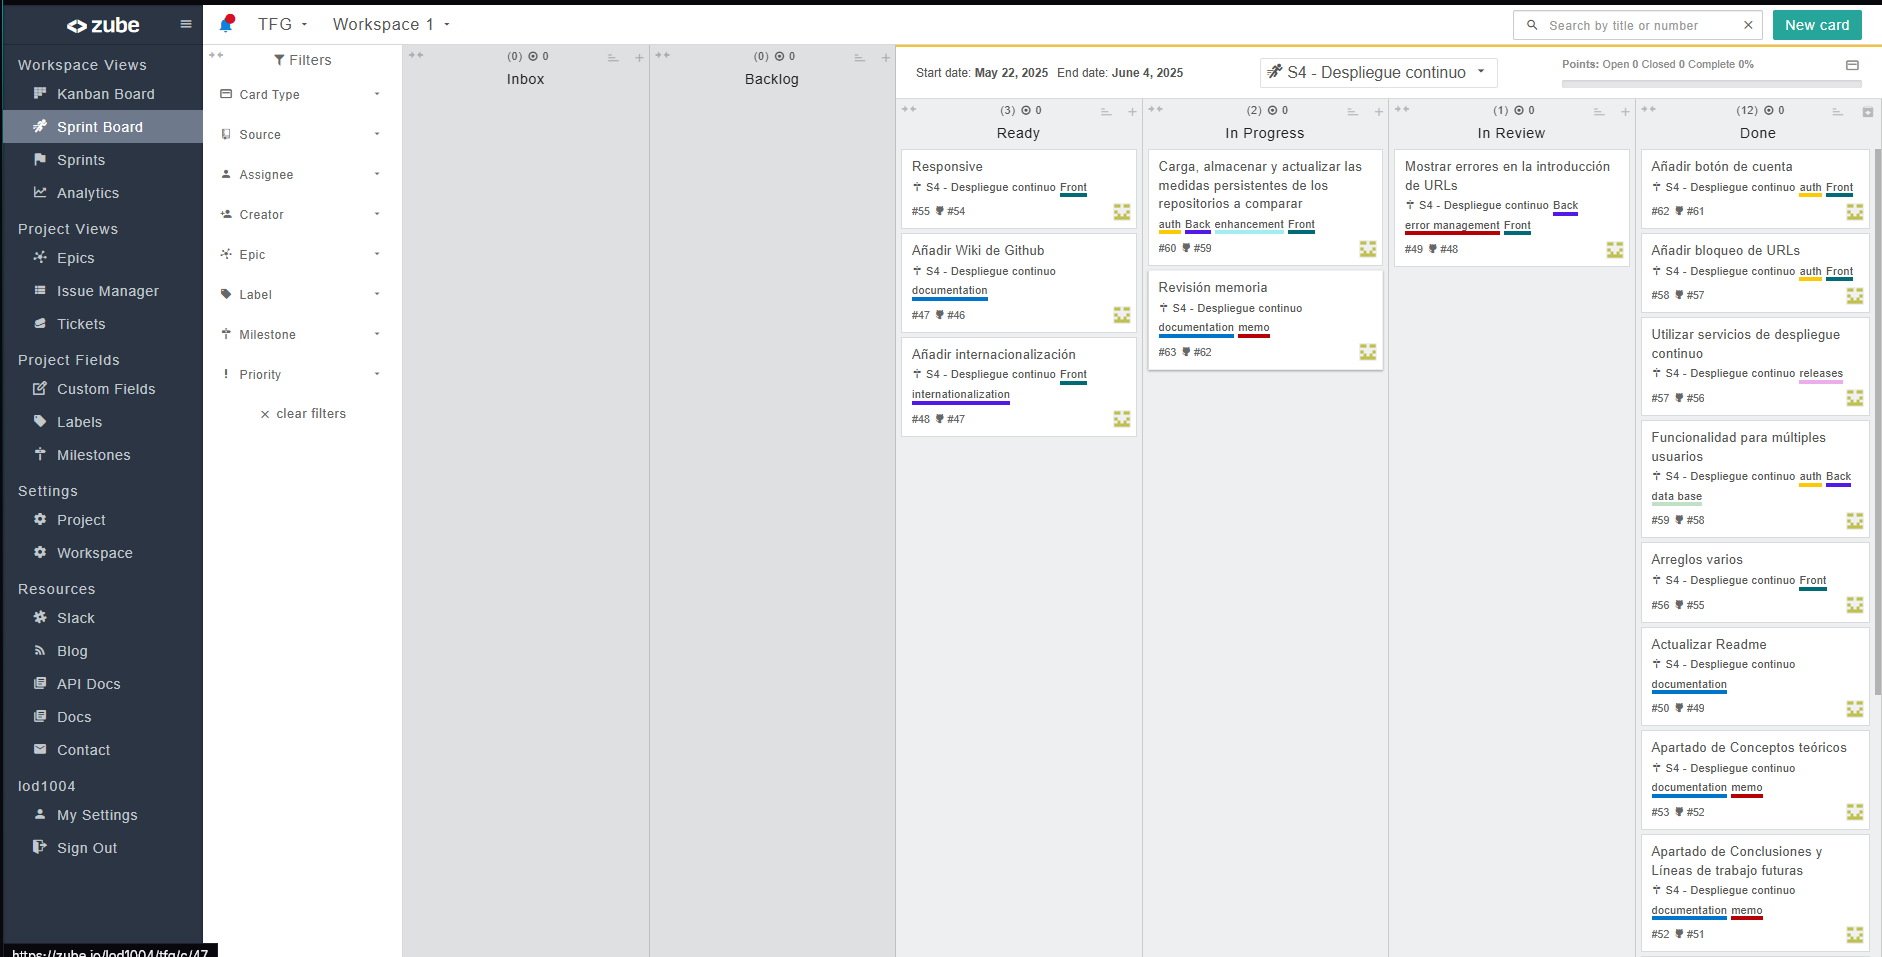
\includegraphics[width=0.8\textwidth]{img/IteracionZube.png}
\caption{Tablero Kanban de la herramienta Zube utilizada para la planificación de tareas e iteraciones.}
\label{fig:zube}
\end{figure}

\section{Tecnologías y herramientas utilizadas}

\subsection{Frontend: Angular}

Para la implementación del cliente se ha optado por el framework \textbf{Angular}, en su versión 19.2.3. Angular ofrece una arquitectura basada en componentes, módulos reutilizables, servicios inyectables y soporte integrado para formularios reactivos. Algunas de sus características más destacadas y útiles en este proyecto han sido:

\begin{itemize}
  \item Formularios reactivos con validación dinámica.
  \item Módulos reutilizables para organizar mejor el código.
  \item Inyección de dependencias para desacoplar lógica y facilitar pruebas.
  \item Integración con bibliotecas como Angular Material para las interfaces de usuario.
\end{itemize}

Se consideraron otras opciones como \textbf{React}, pero se optó por Angular debido a su enfoque más completo y estructurado, más adecuado para una aplicación de análisis con múltiples pantallas y lógica interna, además de la existencia de experiencias previas adquiridas durante las prácticas en empresa en Softeca.

\subsection{Backend: Node.js}

Para el backend se ha utilizado \textbf{Node.js}, un entorno de ejecución para JavaScript que permite desarrollar aplicaciones del lado del servidor de manera eficiente y escalable. Se ha estructurado el servidor como una API REST que recibe peticiones desde el cliente Angular, procesa los datos y devuelve los resultados del análisis.

\begin{itemize}  
  \item \textbf{Modularidad y ecosistema}: Se han utilizado módulos como \texttt{express} para la definición de rutas y controladores, y bibliotecas específicas para consumir APIs de GitHub y procesar datos.
  
  \item \textbf{Facilidad de integración}: Al estar escrito en JavaScript, el backend se integra de forma natural con el frontend desarrollado en Angular, facilitando la comunicación y compartición de lógica o estructuras comunes, lo que facilita el desarrollo.
  
  \item \textbf{Manejo eficiente de errores y validaciones}: Se ha implementado una estructura de control de errores robusta, validación de parámetros de entrada, y respuestas claras al cliente ante peticiones incorrectas o fallos del análisis.
\end{itemize}

Se consideraron otras alternativas como Python (con frameworks como FastAPI o Flask), pero se optó por Node.js por su rapidez de desarrollo, la familiaridad con el lenguaje y su amplia adopción en aplicaciones web modernas.

\subsection{Comunicación cliente-servidor}

La comunicación entre el cliente Angular y el backend FastAPI se realiza a través de peticiones HTTP RESTful, usando el módulo \texttt{HttpClient} de Angular. La respuesta del backend incluye las medidas de proceso en los repositorios a analizar y a evaluar a partir de los repositorios de referencia proporcionados por el usuario.

\subsection{Base de datos: MongoDB y MongoDB Compass}

Para el almacenamiento de información relacionada con los análisis realizados y la persistencia de datos relevantes, se ha utilizado \textbf{MongoDB}, una base de datos NoSQL orientada a documentos. Esta elección se debe a su flexibilidad, escalabilidad y facilidad de uso con Node.js.

\begin{itemize}
  \item \textbf{Modelo de documentos}: MongoDB permite trabajar con documentos en formato JSON, lo cual se adapta perfectamente a los datos semiestructurados obtenidos del análisis de los repositorios de GitHub.
  
  \item \textbf{Integración con Node.js}: Se ha utilizado la biblioteca \texttt{mongoose} para gestionar la conexión, definición de esquemas y operaciones con la base de datos desde el backend Node.js, facilitando el trabajo con modelos y validaciones.
  
  \item \textbf{Visualización y gestión con MongoDB Compass}: Para la gestión visual y análisis manual de los datos almacenados se ha utilizado \textbf{MongoDB Compass}, una interfaz gráfica que permite explorar documentos, ejecutar consultas, y visualizar estadísticas de uso de la base de datos de forma sencilla e intuitiva.
  
\end{itemize}

La elección de MongoDB frente a bases de datos relacionales como MySQL o PostgreSQL se justifica por la naturaleza no estructurada de los datos analizados y la necesidad de una estructura flexible que pueda evolucionar fácilmente sin migraciones complejas, además se su buena integración con el backend Node. js.


\subsection{Diseño de la interfaz de usuario}

Se ha utilizado la biblioteca \textbf{Angular Material} para implementar una interfaz moderna y coherente visualmente. Esta biblioteca proporciona componentes reutilizables (botones, tablas, inputs, spinners, etc.) con accesibilidad integrada y estilos basados en Material Design.

El diseño se ha centrado en la claridad y la simplicidad, mostrando los resultados del análisis de manera visual e intuitiva, junto con retroalimentación clara (colores, iconos, puntuaciones) para ayudar al usuario a interpretar los resultados.

\subsection{Gestión del código fuente}

El código fuente del proyecto se ha gestionado con \textbf{Git}, utilizando GitHub como repositorio remoto. Se ha trabajado con ramas para separar funcionalidades y mantener el código estable en la rama principal.

\subsection{Despliegue continuo de la aplicación web durante el desarrollo}

Para las pruebas de aceptación del tutor y el desarrollo del proyecto se han utilizado dos herramientas: Render y Vercel. Estas herramientas han permitido el despliegue continuo de la aplicación web a través de la integración continua lograda gracias a la compatibilidad entre estas dos herramientas y el repositorio de GitHub donde se ha ido subiendo el código del backend y el frontend

\begin{itemize}
  \item \textbf{Despliegue continuo del backend}: Se ha utilizado la herramienta de Render para lograr el despliegue continuo del backend desde el repositorio de GitHub
  
  \item \textbf{Despliegue continuo del frontend}: Para el frontend se ha utilizado la herramienta de Vercel, que permite un despliegue continuo rápido y eficiente, que se puede probar desde cualquier dispositivo por cualquier persona gracias a la opción de usar despliegues de carácter público.
  
\end{itemize}

Estas herramientas de despliegue han mejorado la comunicación y las pruebas de aceptación tanto al tutor como a diferentes usuarios que han ayudado al desarrollo de la aplicación web y a la búsqueda de errores.

\section{Otras herramientas de apoyo}

\begin{itemize}
  \item \textbf{Visual Studio Code}: Editor principal usado para escribir tanto el frontend como el backend.
  \item \textbf{LaTeX}: Utilizado para la redacción de esta memoria, por su capacidad de estructurar documentos técnicos de manera clara y profesional.
  \item \textbf{Zube}: Para documentar el código, organizar las tareas de desarrollo y las decisiones técnicas dentro del propio repositorio se ha utilizado la herramienta de Zube, recomendada por el profesor y conectada con el repositorio de GitHub.
  \item \textbf{GitHub Desktop}: Herramienta gráfica de GitHub que permite visualizar claramente los cambios realizados en todo el repositorio de forma individual y comparativa antes de subir todos los cambios con un solo Commit.
  
\end{itemize}

\section{Comparativa de tecnologías evaluadas}

Durante la fase inicial del proyecto se analizaron distintas tecnologías. Las siguientes tablas resume los principales aspectos que se compararon:

\begin{center}
\begin{tabular}{|l|c|c|c|}
\hline
\textbf{Tecnología} & \textbf{Facilidad de uso} & \textbf{Rendimiento} & \textbf{Documentación} \\
\hline
Angular & Alta & Media-Alta & Muy completa \\
React & Media & Alta & Muy completa \\
Vue & Alta & Media & Buena \\
FastAPI & Alta & Alta & Muy completa \\
Flask & Alta & Media & Muy completa \\
Django & Media & Media & Muy completa \\
\hline
\end{tabular}
\captionof{table}{Comparativa de tecnologías frontend y backend evaluadas en la fase inicial del proyecto.}
\end{center}

\begin{center}
\begin{tabular}{|l|c|c|c|}
\hline
\textbf{Tecnología} & \textbf{Facilidad de uso} & \textbf{Rendimiento} & \textbf{Documentación} \\
\hline
Node.js & Media-Alta & Alta & Muy completa \\
Express.js & Alta & Alta & Muy completa \\
FastAPI & Alta & Alta & Muy completa \\
Flask & Alta & Media & Muy completa \\
Django & Media & Media & Muy completa \\
Spring Boot & Baja & Muy Alta & Muy completa \\
\hline
\end{tabular}
\captionof{table}{Comparativa de tecnologías backend y frameworks analizados.}
\end{center}


\begin{center}
\begin{tabular}{|l|c|c|c|}
\hline
\textbf{Base de Datos} & \textbf{Facilidad de uso} & \textbf{Rendimiento} & \textbf{Documentación} \\
\hline
MongoDB & Alta & Alto (NoSQL) & Muy completa \\
MySQL & Medio-Alta & Alto & Muy completa \\
PostgreSQL & Media & Muy Alto & Muy completa \\
SQLite & Alta & Medio-Bajo & Buena \\
Firebase Realtime DB & Muy alta & Medio & Buena \\
Redis & Media & Muy Alto (caché) & Buena \\
\hline
\end{tabular}
\captionof{table}{Comparativa de tecnologías de bases de datos utilizadas y evaluadas.}
\end{center}


La elección final se basa en la compatibilidad entre tecnologías, la curva de aprendizaje, y el tipo de aplicación (analítica, con formularios complejos y visualización estructurada).

\section{Resumen de herramientas utilizadas}

A continuación se muestra una tabla con las herramientas utilizadas durante el proceso de desarrollo de software del proyecto, junto con la indicación de a qué parte del proceso corresponden

\begin{table}[H]
\centering
\caption{Herramientas y tecnologías utilizadas en cada parte del proyecto.}
\label{herramientasportipodeuso}
\begin{tabular}{l c c c c c}
\toprule
\textbf{Herramientas} & Frontend & Backend & Base de Datos & Documentación & Despliegue \\
\midrule
HTML5 & X & & & & \\
TypeScript & X & & & & \\
Angular 19.2.3 & X & & & & \\
Node.js & & X & & & \\
XP & & X & & & \\
GitHub API & & X & & & \\
Mongoose & & X & X & & \\
MongoDB & & & X & & \\
MongoDB Compass & & & X & & \\
JWT & & X & & & \\
Render & & X & & & X \\
Vercel & X & & & & X \\
\LaTeX{} & & & & X & \\
Overleaf & & & & X & \\
Git & X & X & X & X & X \\
\bottomrule
\end{tabular}
\end{table}
\capitulo{5}{Aspectos relevantes del desarrollo del proyecto}

Durante la implementación de este Trabajo de Fin de Grado, se han tomado decisiones técnicas y de diseño que han marcado de forma clara el rumbo y la calidad final del proyecto \textit{Asistente de prácticas ágiles para repositorios en GitHub}. Este capítulo describe los aspectos más destacados del desarrollo, sus motivaciones y las soluciones adoptadas, con el objetivo de que puedan servir de referencia para otros estudiantes o desarrolladores que se enfrenten a retos similares.

\section{Motivación para el proyecto}
Desde el principio la idea del proyecto era asistir al usuario al desarrollo de la creación de trabajos en repositorios de GitHub, pero no al código de los trabajos, si no al repositorio en sí. En GitHub hay un montón de herramientas y opciones que pasan desapercibidas, especialmente para estudiantes de la carrera de Ingeniería Informática que no tienen tanta experiencia con esta plataforma. Muchos hacen proyectos enteros sin saber siquiera lo que es una Issue, una Release, que pueden agregar implementación continua usando GitHub Actions, etc. Por ello se decidió que en este Trabajo de Fin de Grado se desarrollaría una aplicación que ayudara al desarrollo de repositorios en el ámbito docente para facilitiar y agilizar la planificación trabajo de los estudiantes en GitHub.

\section{Prácticas Ágiles como base teórica}

Para ayudar a los usuarios a trabajar con sus repositorios necesitaríamos unas bases teóricas que ayudaran a justificar el por qué de los resultados que la aplicación proporcionaría, y finalmente se eligieron las prácticas Ágiles, un concepto con el que los estudiantes del Grado de Ingeniería Informática están familiarizados, especialmente por la asignatura del tercer curso \textbf{Gestíon de Proyectos}. Finalmente se así decidió mostrar los resultados de los análisis de los repositorios en forma de prácticas de agilidad sacadas del Agile Subway Map \cite{agileSubwayMap} como Integración Continua, Control de Versiones, etc. Estas prácticas evalúan aspectos como la frecuencia de commits, la coherencia en los mensajes, la asignación de issues, y la distribución del trabajo.

Posteriormente se desarrolló un módulo de evaluación de estas prácticas que, a partir de los datos obtenidos vía la API de GitHub, genera una puntuación por cada práctica y un resumen visual en el FrontEnd que permite observar tanto rápidamente los puntos fuertes y débiles del repositorio, como detalladamente las bases teóricas de la práctica Ágil que se cumplen o no, explicando el por qué. Esta funcionalidad fue clave para transformar el análisis en una herramienta útil para no solo estudiantes, sino también profesores o equipos de desarrollo.

\section{La tecnología de Node js y Angular} Se optó por usar la tecnología de Angular para el FrontEnd por su gran capacidad para diseñar aplicaciones web eficaces, fáciles de maquetar y estilizar, y gran variedad de herramientas como servicios, componentes, módulos, y librerías que ayudan a desarrollar fácilmente una aplicación totalmente funcional y agradable al usuario. Previamente a este proyecto ya había trabajado en varias aplicaciones que usaban esta tecnología, lo cual ayudó desde un comienzo a tener clara la estructura de esta parte del código.

También se optó por usar Node js en el BackEnd debido a la similaridad del lenguaje (JavaScript) con el que usa Angular para sus componentes que implementan la funcionalidad del código (TypeScript).

Estas decisiones permitieron generar un ejecutable funcional, autocontenible y sin dependencias externas, mejorando la portabilidad y experiencia del usuario final.

\section{Selección de MongoDB como sistema de almacenamiento}

MongoDB fue elegido como base de datos por su naturaleza flexible y su excelente integración con Node.js y su facilidad de uso. Además, al tratarse de una aplicación local, se optó por una base de datos embebida que no requiriese configuración externa por parte del usuario.

\section{Arquitectura modular y comunicación entre capas}

La aplicación se estructura en tres capas claramente diferenciadas: BackEnd (Node.js), base de datos (MongoDB) y FrontEnd (Angular)). Esta separación permitió trabajar en cada módulo de manera independiente y facilitó la escalabilidad del sistema.

El BackEnd ofrece una API REST con rutas específicas para analizar repositorios, extraer estadísticas y aplicar prácticas basadas en prácticas ágiles, todo esto guardando los resultados en una base de datos en MONGODB, de la cual extraerlos posteriormente para mandarlos al FrontEnd una vez se requieran a través de diferentes llamadas y joins. Por su parte, el FrontEnd permite al usuario interactuar de forma visual, seleccionando repositorios, rangos de fechas y recibiendo evaluaciones contextualizadas. La comunicación se realiza mediante peticiones HTTP sobre \texttt{localhost}, garantizando así una experiencia fluida sin requerir conexión a internet.

\section{Integración de lenguaje natural para resúmenes y explicaciones}

Con el objetivo de ofrecer una experiencia más didáctica y comprensible, se exploró el uso de modelos de lenguaje (LLM) para generar explicaciones en lenguaje natural a partir de los resultados del análisis. 

Inicialmente se evaluaron opciones como OpenAI GPT y modelos open-source, priorizando la claridad y la coherencia en las respuestas. Finalmente, debido a que la mayoría de mensajes de resultado que aparecerían tras el análisis serían similares estructuralmente y bastante cortos dentro de lo posible, se decidió que como posible mejora del sistema, se podría integrar una capa de generación de lenguaje que permita resumir los informes y ofrecer feedback personalizado.

\section{Desarrollo iterativo y depuración mediante testing manual}

Dado el alcance de la aplicación y su complejidad funcional, se adoptó un enfoque de desarrollo iterativo. Cada módulo (visualización, análisis, integración con GitHub, etc.) fue construido y probado individualmente a través de la basede datos de Mongo y la consola del BackEnd antes de su integración global.

Uno de los principales retos cerca del final del proyecto fue la depuración en entorno empaquetado. Al final se optó por lanzar las releases en forma de BackEnds empaquetados que accederían al FrontEnd y a las variables de entorno en la misma carpeta y, por motivos de calidad, sería necesario insertar registros de log visibles en pantalla o mediante archivos para detectar errores silenciosos, así como el progreso de análisis de repositorios de la aplicación.

\section{Autoformación y búsqueda activa de soluciones}

El proyecto ha supuesto un esfuerzo significativo de aprendizaje autónomo en varias tecnologías: Angular, Node js, MongoDB o GitHub REST API. Muchos de los problemas encontrados fueron resueltos consultando documentación oficial, foros técnicos (como Stack Overflow o GitHub Issues), recursos especializados, o comparándolos con problemas similares tenidos en proyectos previos (Especialmente en la parte del FrontEnd en Angular).

\capitulo{6}{Trabajos relacionados}

\section{Documentación de la evolución de proyectos en el tiempo}

Uno de los aspectos diferenciales del presente proyecto frente a herramientas similares es su capacidad para analizar la evolución temporal de los repositorios software. Esta funcionalidad permite al usuario seleccionar rangos de fechas personalizados sobre los cuales se calcularán las métricas, facilitando así el seguimiento detallado del progreso, mantenimiento y salud de un proyecto a lo largo del tiempo. Esta característica no está presente en muchas de las herramientas analizadas, donde los análisis se realizan de forma estática y centrados en el estado actual del repositorio.

Gracias a esta funcionalidad temporal, el usuario puede, por ejemplo, evaluar cómo ha cambiado la calidad del repositorio desde el inicio del mismo, o comprobar si el uso de las prácticas ágiles de desarrollo han tenido impacto en la velocidad y el desarrollo del mismo. Esta capacidad resulta especialmente útil en contextos docentes (como proyectos fin de carrera o asignaturas de carreras relacionadas a la informática), donde se requiere un seguimiento detallado y didáctico de la evolución del trabajo de los estudiantes.

Además, incluye la posibilidad de realizar tanto análisis relativos como análisis absolutos, algo poco común en herramientas similares. Esto permite no sólo se observar si un repositorio mejora o empeora con el paso de unidades de tiempo, si no también con el paso de las distintas fases de desarrollo del proyecto. Por ejemplo, se puede observar si la definición de "Done" se respeta de forma más consistente con el paso de los sprints, o si las prácticas de integración continua se estabilizan a lo largo de los meses.

Esta funcionalidad no se recoge en otras herramientas como \textit{Criticality-Score}, \textit{Agile-Metrics} o \textit{Activity-API}, las cuales realizan análisis puntuales y no permiten al usuario especificar periodos temporales personalizados. Los tres proyectos mencionados abordan el análisis de proyectos de software desde distintas perspectivas, sirviendo como referentes valiosos para el desarrollo del presente trabajo. 

Criticality-Score se centra en medir la importancia de los proyectos open source para priorizar su seguridad, pero no evalúa métricas cualitativas ni trabaja con umbrales.

Agile-Metrics recopila indicadores ágiles según la forja de repositorio utilizada, pero carece de una unificación de métricas y no trabaja con GitHub o GitLab, lo que limita su alcance. 

Activity-API, más cercano al proyecto presentado en esta memoria, permite evaluar y comparar métricas de actividad, aunque sólo entre dos proyectos. 

En conjunto, estos proyectos ofrecen ideas complementarias, pero el actual amplía sus funcionalidades con una mayor capacidad de comparación y evaluación de métricas mediante intervalos temporales, resultando así en una herramienta avanzada tanto para análisis retrospectivos en detalle como para evaluación continua durante el desarrollo..
\capitulo{7}{Conclusiones y Líneas de trabajo futuras}

Todo proyecto debe incluir las conclusiones que se derivan de su desarrollo. Éstas pueden ser de diferente índole, dependiendo de la tipología del proyecto, pero normalmente van a estar presentes un conjunto de conclusiones relacionadas con los resultados del proyecto y un conjunto de conclusiones técnicas. 
Además, resulta muy útil realizar un informe crítico indicando cómo se puede mejorar el proyecto, o cómo se puede continuar trabajando en la línea del proyecto realizado. 



\bibliographystyle{plain}
\bibliography{bibliografia}

\end{document}

% Introducción
\newpage
\section{Introducción}
Placeholder

\end{document}
